\documentclass[aspectratio=169]{beamer}

\usepackage{mathtools}
\usepackage{graphicx}
\usepackage{tikz}
\usetheme{Szeged}

\newcommand{\code}[1]{\underline{#1}}
\newcommand{\prog}[1]{\textsf{\bfseries #1}}

\setbeamertemplate{navigation symbols}{}
\definecolor{ialred}{rgb}{0.73,0.11,0.11}
\definecolor{searchblue}{rgb}{0.38,0.65,0.98}

\usecolortheme[named=searchblue]{structure}
\setbeamercolor{titlelike}{fg=white,bg=searchblue}

\title[IDI Search]{\textbf{IDI Search}\\
    \textit{A metadata search app for exploring\\New Zealand’s administrative linked data}
}

\author{Tom Elliott\texorpdfstring{\\[0.5em]}{and}
    \textbf{\scriptsize Collaborators}\texorpdfstring{\\}{:}
    \footnotesize Barry Milne, Eileen Li, Andrew Sporle, and Colin Simpson
}
\institute[Te Rourou Tātaritanga / iNZight Analtytics Ltd]{
    Developed by: Te Rourou Tātaritanga \, {\color{gray} terourou.org}\texorpdfstring{\\}{,}
    Ongoing support: iNZight Analytics Ltd \, {\color{gray} inzight.co.nz}
}

\titlegraphic{\vspace{-6.5em}\hspace{-28em}
   
\includegraphics[width=2cm]{idisearch}
}

\date{IPDLN Chicago\linebreak September 2024}


\begin{document}


\setbeamertemplate{headline}{}
\setbeamertemplate{footline}{}
\begin{frame}
    \vspace{-2.5em}
    \maketitle
\end{frame}

\setbeamertemplate{headline}[miniframes theme]
\setbeamertemplate{footline}[miniframes theme]

\section{Introduction}

\begin{frame}
    \frametitle{The Integrated Data Infrastructure (IDI)}

    \begin{columns}
    \begin{column}{0.5\textwidth}
        \begin{center}
            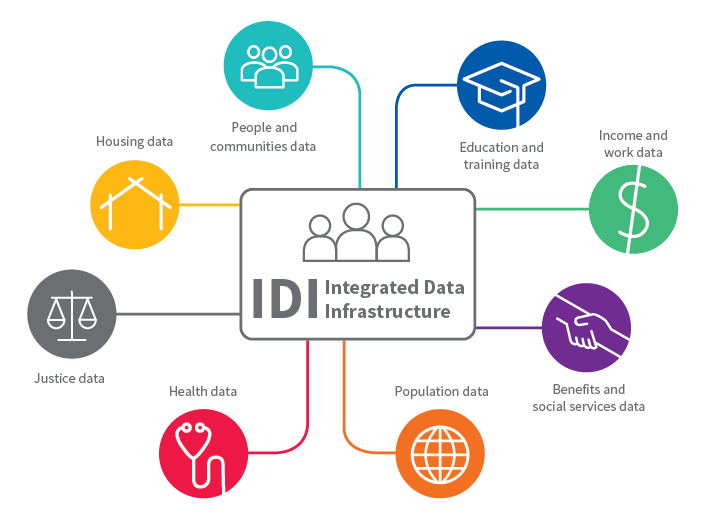
\includegraphics[width=\linewidth]{idi.png}
        \end{center}
    \end{column}
    \begin{column}{0.5\textwidth}
        % \begin{itemize}
            An integrated database containing de-identified longitudinal microdata about people, households, \& businesses.
        % \end{itemize}
    \end{column}
    \end{columns}
\end{frame}


\begin{frame}
    \frametitle{What's in the IDI?}

    \begin{itemize}
        \item $\approx{}50,000$ variables, $\approx{}1,000$ datasets
        \item Government agencies, surveys, and non-government organisations
        \item Linkable at the individual level
    \end{itemize}

\end{frame}


\begin{frame}
    \frametitle{The problem: access to metadata}

    \begin{itemize}
        \item Data dictionaries contain metadata about collections of datasets
        \item Independent maintenance across agencies
        \begin{itemize}
            \item Inconsistencies, typos, etc.
            \item Duplication
        \end{itemize}
        \item Only available to approved, existing researchers
        \item Not easily navigable, difficult to keep up with changes
    \end{itemize}
\end{frame}

\section{Creating a solution}

\begin{frame}
    \frametitle{Why a search app?}

    \begin{itemize}
        \item A publicly available, searchable database
        \item What data is available?
        \item What has changed?\\[2em]

        \item[$\Rightarrow$] Increase utility of a valuable database
    \end{itemize}
\end{frame}


\begin{frame}
    \frametitle{Data sources}

    \begin{itemize}
        \item Database schema
        \item Data dictionaries
        \item Manually curated metadata
        \begin{itemize}
            \item Agency names and associated collections
            \item Renamed datasets/variables
            \item Datestamped tables
        \end{itemize}
    \end{itemize}
\end{frame}

\begin{frame}
    \frametitle{Read data dictionaries}

    \begin{columns}
        \begin{column}{0.5\textwidth}
        \begin{center}
            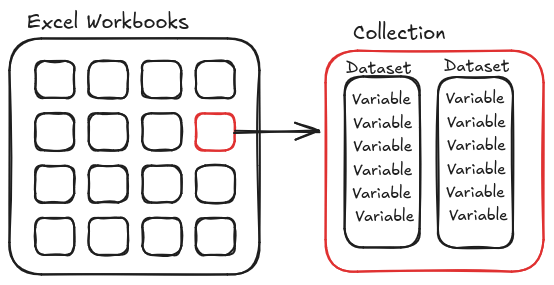
\includegraphics[width=\linewidth]{dd-workflow.png}
        \end{center}
        \includegraphics[width=0.2\linewidth]{rlogo.png}
    \end{column}

    \begin{column}{0.5\textwidth}
        \begin{itemize}
            \item Search workbook for keywords
            \item Sanitise data
            \begin{itemize}
                \item Minor errors fixed
                \item Otherwise rejected
            \end{itemize}
            \item Returned to Stats NZ (usually fixed!)
        \end{itemize}

    \end{column}
    \end{columns}
\end{frame}

\begin{frame}
    \frametitle{Read SQL variable list}

    \begin{columns}
        \begin{column}{0.5\textwidth}
            \begin{center}
                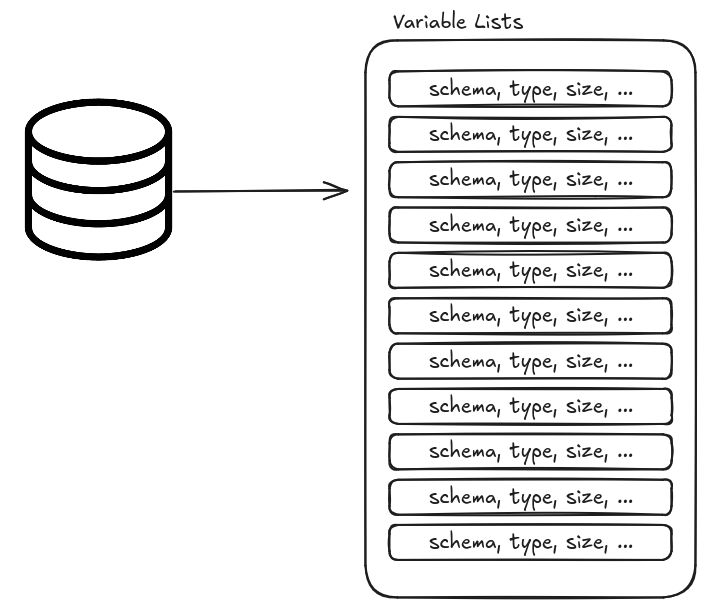
\includegraphics[width=0.8\linewidth]{dd-sql.png}
            \end{center}
        \end{column}
        \begin{column}{0.5\textwidth}
            \begin{itemize}
                \item Stats NZ generate at each update
                \item Standard IDI output process
            \end{itemize}
        \end{column}
    \end{columns}

\end{frame}

\begin{frame}
    \frametitle{Combine with metadata}

    \begin{columns}
        \begin{column}{0.5\textwidth}
            \begin{center}
                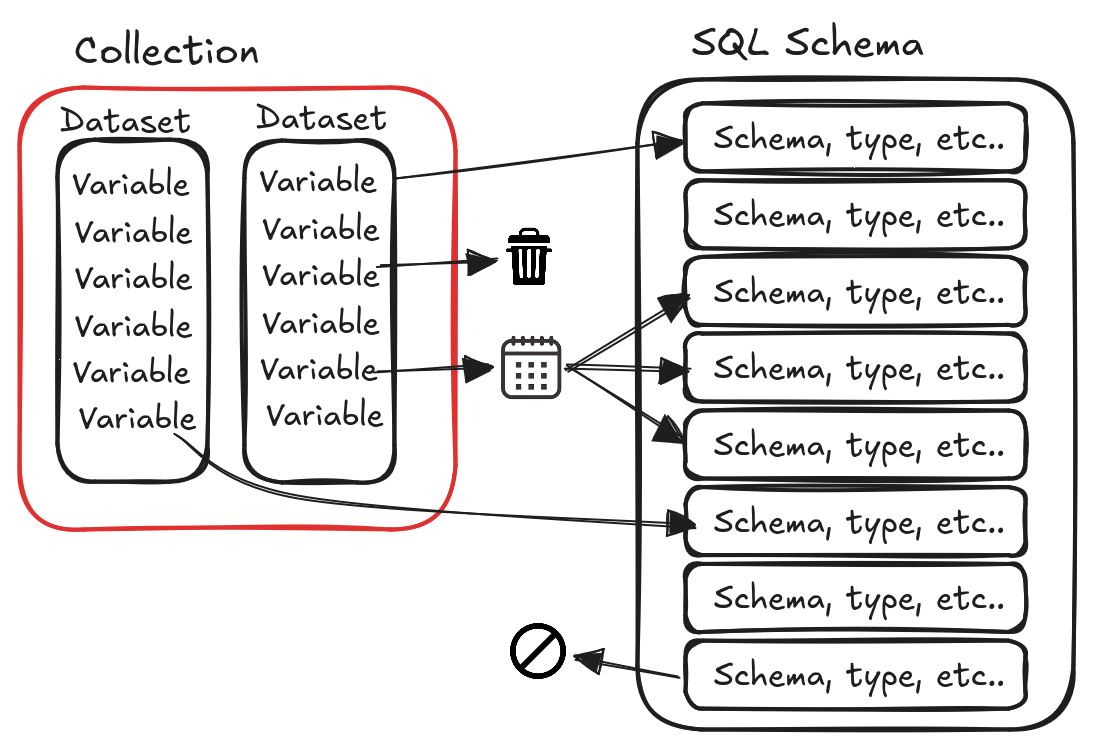
\includegraphics[width=0.8\linewidth]{dd-merge.png}
            \end{center}
        \end{column}
        \begin{column}{0.5\textwidth}
            \begin{itemize}
                \item Variables missing from dictionaries
                \item Variables deleted from IDI (or error)
                \item Datestamped variables
            \end{itemize}
        \end{column}
    \end{columns}

\end{frame}

\begin{frame}
    \frametitle{Final clean data}

    \begin{center}
        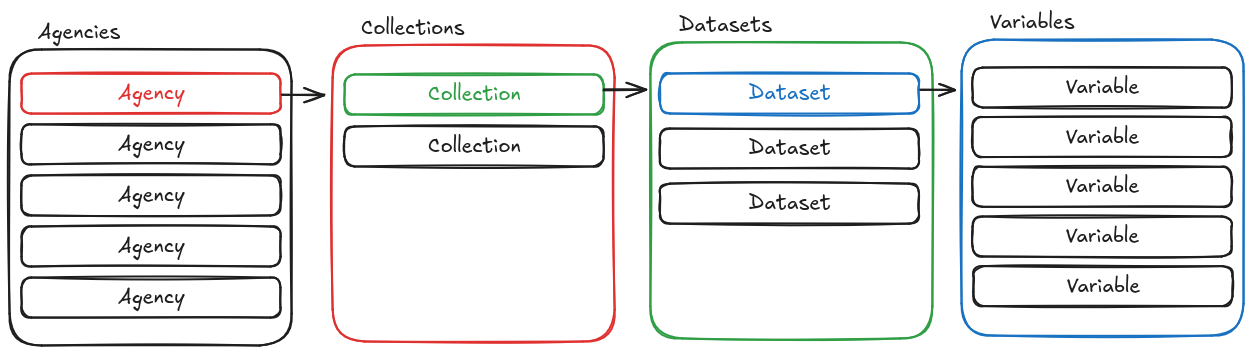
\includegraphics[width=0.7\linewidth]{dd-result.png}
    \end{center}

    \begin{itemize}
        \item Text fields cleaned/formatted
        \item Duplicates removed
        \item Written to MySQL database
    \end{itemize}

\end{frame}

\section{IDI Search}

\begin{frame}
    \frametitle{Deployed solution: IDI Search app}

    \begin{columns}
        \begin{column}{0.5\textwidth}
            \begin{center}
                
\includegraphics[width=0.5\linewidth]{idisearch.png}
            \end{center}
        \end{column}
        \begin{column}{0.5\textwidth}
            \begin{itemize}
                \item UI: NextJS (Javascript framework)
                \item MySQL text search
                \item Cross-linking for easy navigation
                \item \url{idisearch.terourou.org}
            \end{itemize}
        \end{column}
    \end{columns}

\end{frame}

{ % all template changes are local to this group.
\setbeamertemplate{navigation symbols}{}
\begin{frame}<article:0>[plain]
    \begin{tikzpicture}[remember picture,overlay]
        \node[at=(current page.center)] {
            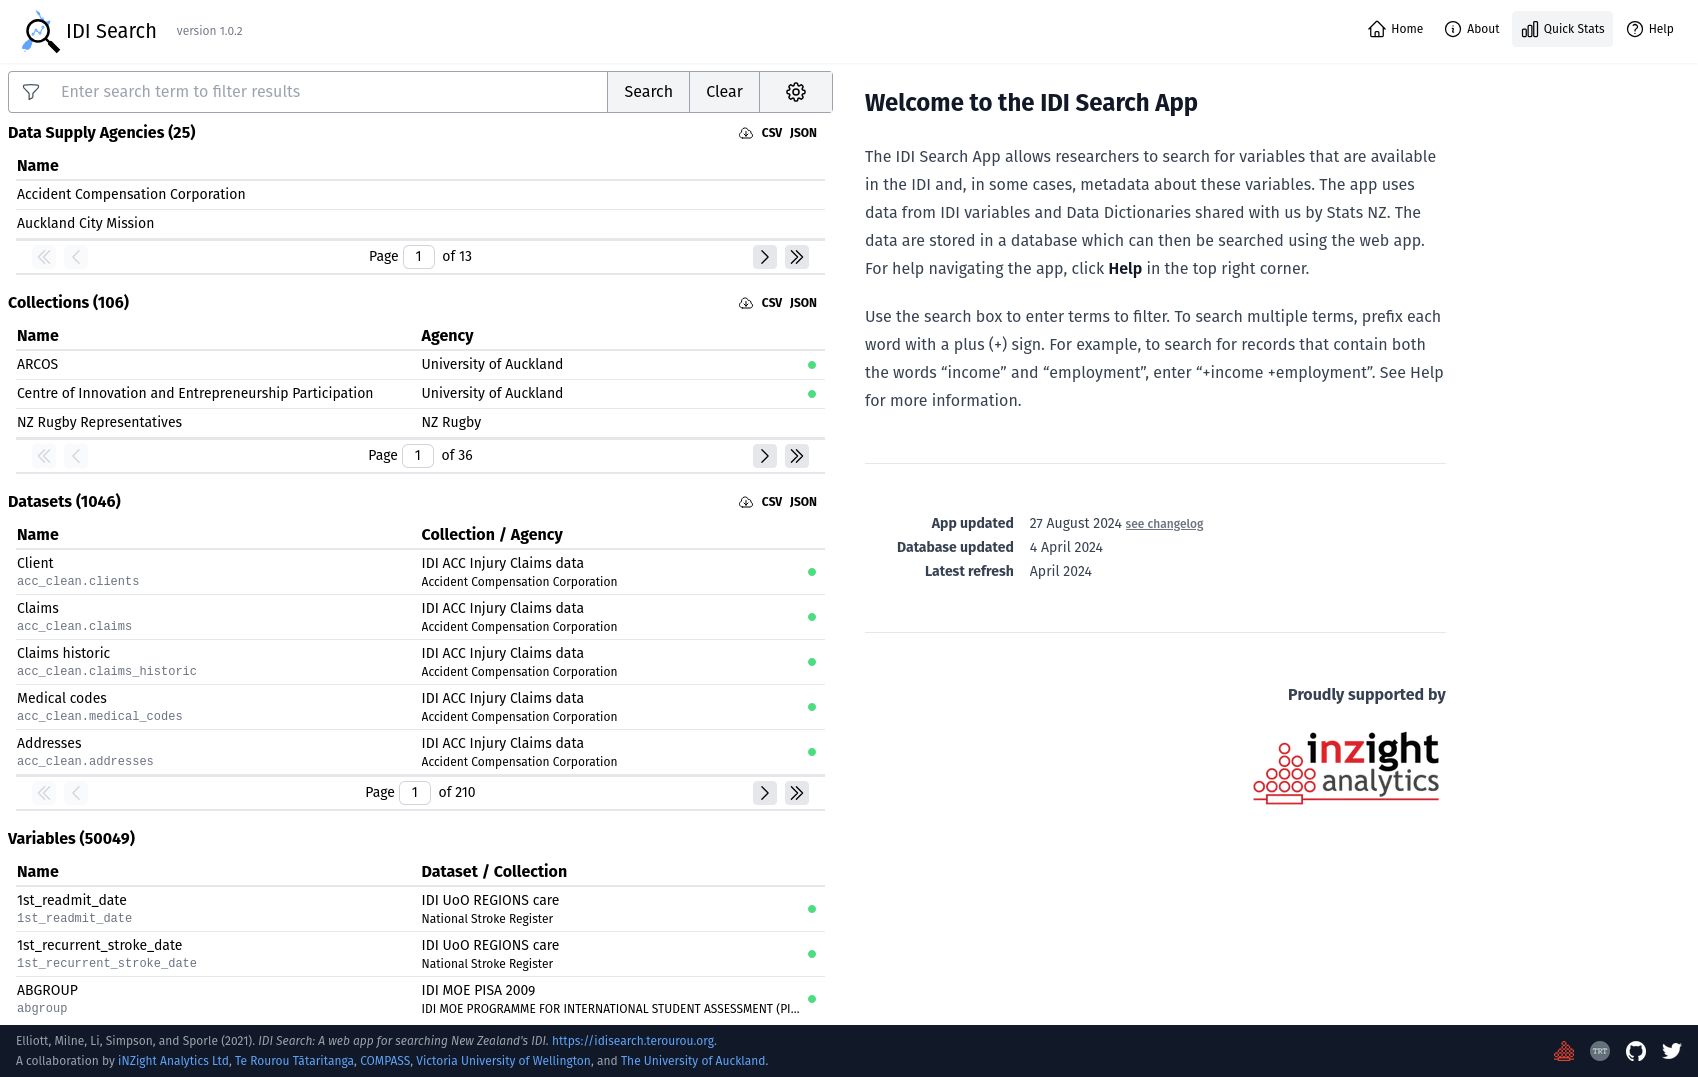
\includegraphics[keepaspectratio,
            width=\paperwidth,
            height=\paperheight]{demo1.png}
            };
    \end{tikzpicture}
\end{frame}
\begin{frame}<article:0>[plain]
    \begin{tikzpicture}[remember picture,overlay]
        \node[at=(current page.center)] {
            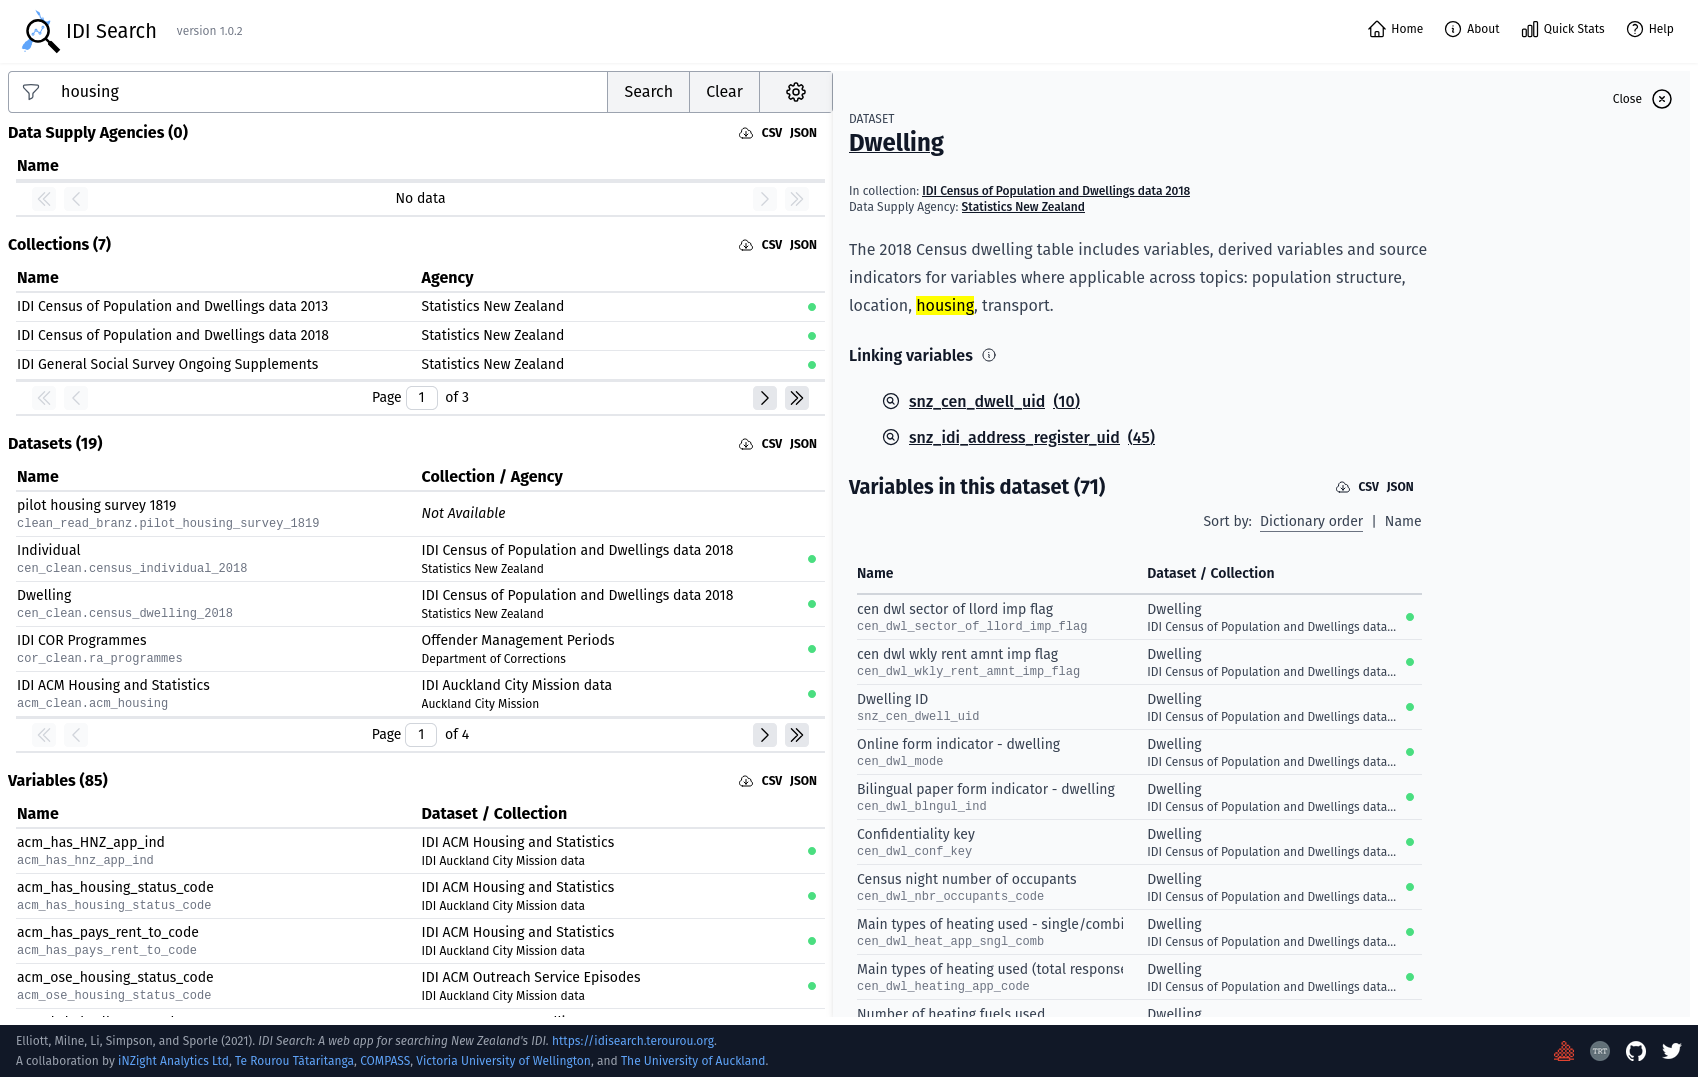
\includegraphics[keepaspectratio,
            width=\paperwidth,
            height=\paperheight]{demo2.png}
            };
    \end{tikzpicture}
\end{frame}
\begin{frame}<article:0>[plain]
    \begin{tikzpicture}[remember picture,overlay]
        \node[at=(current page.center)] {
            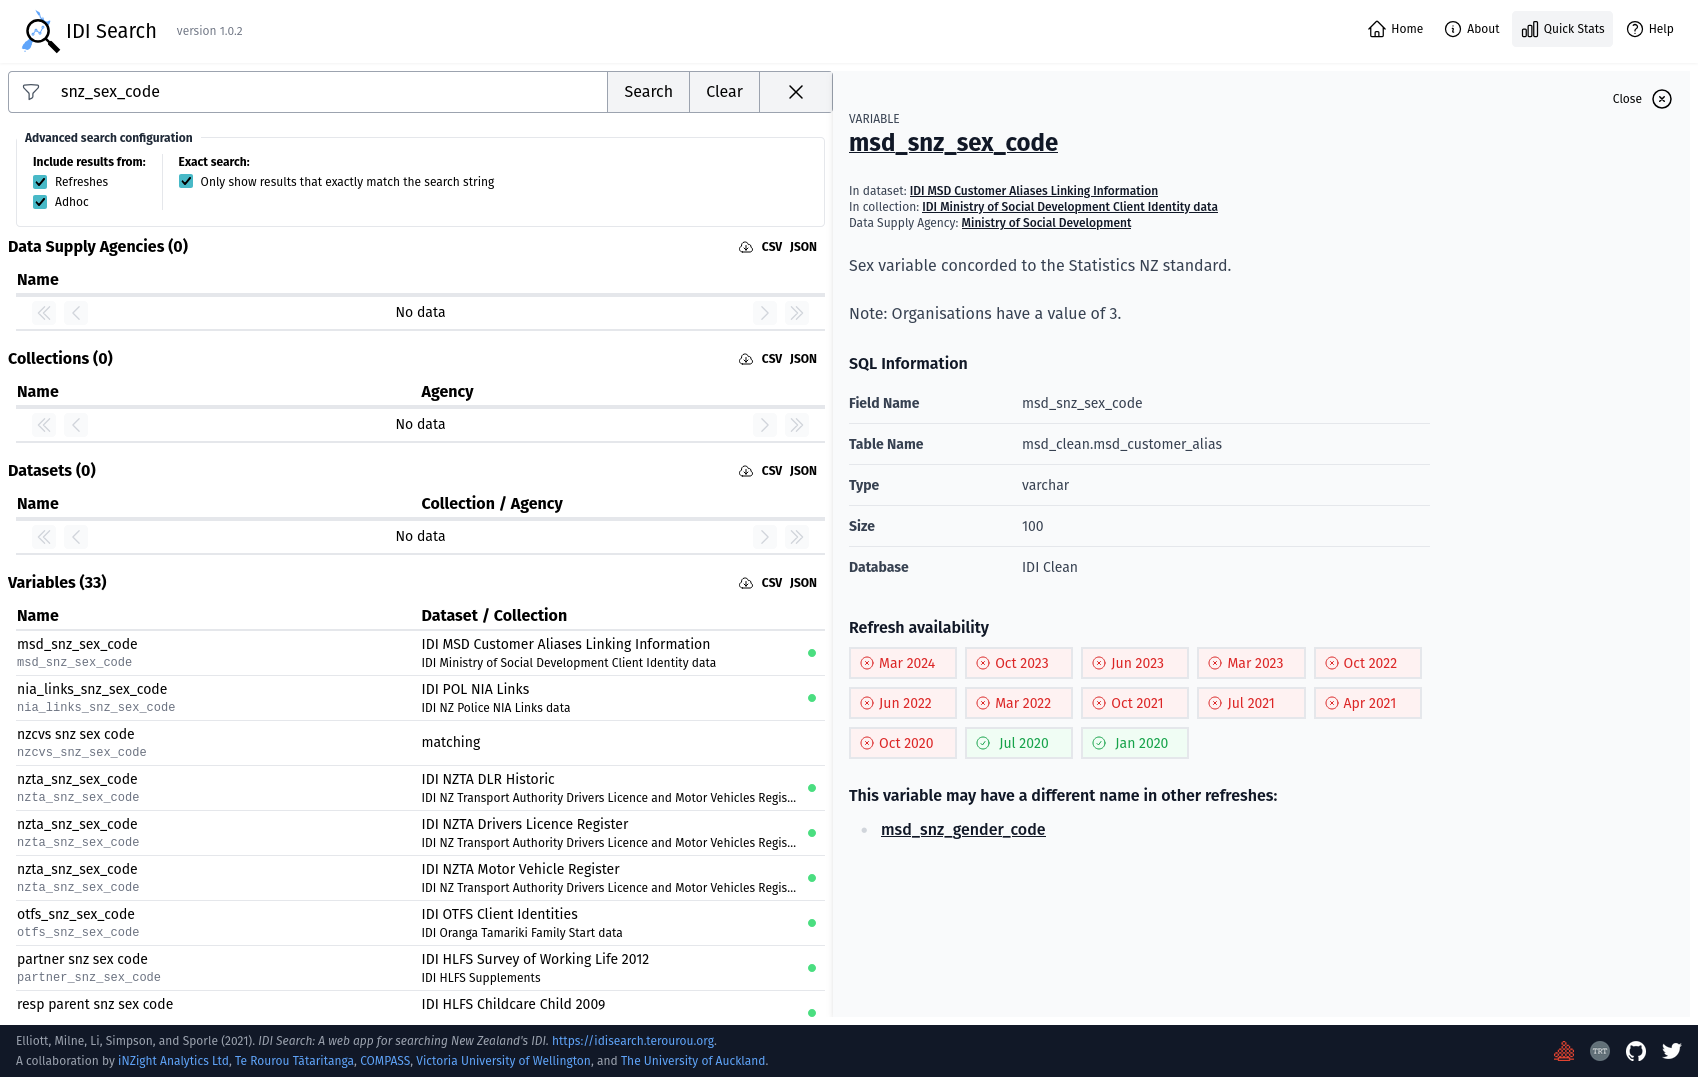
\includegraphics[keepaspectratio,
            width=\paperwidth,
            height=\paperheight]{demo3.png}
            };
    \end{tikzpicture}
\end{frame}
\begin{frame}<article:0>[plain]
    \begin{tikzpicture}[remember picture,overlay]
        \node[at=(current page.center)] {
            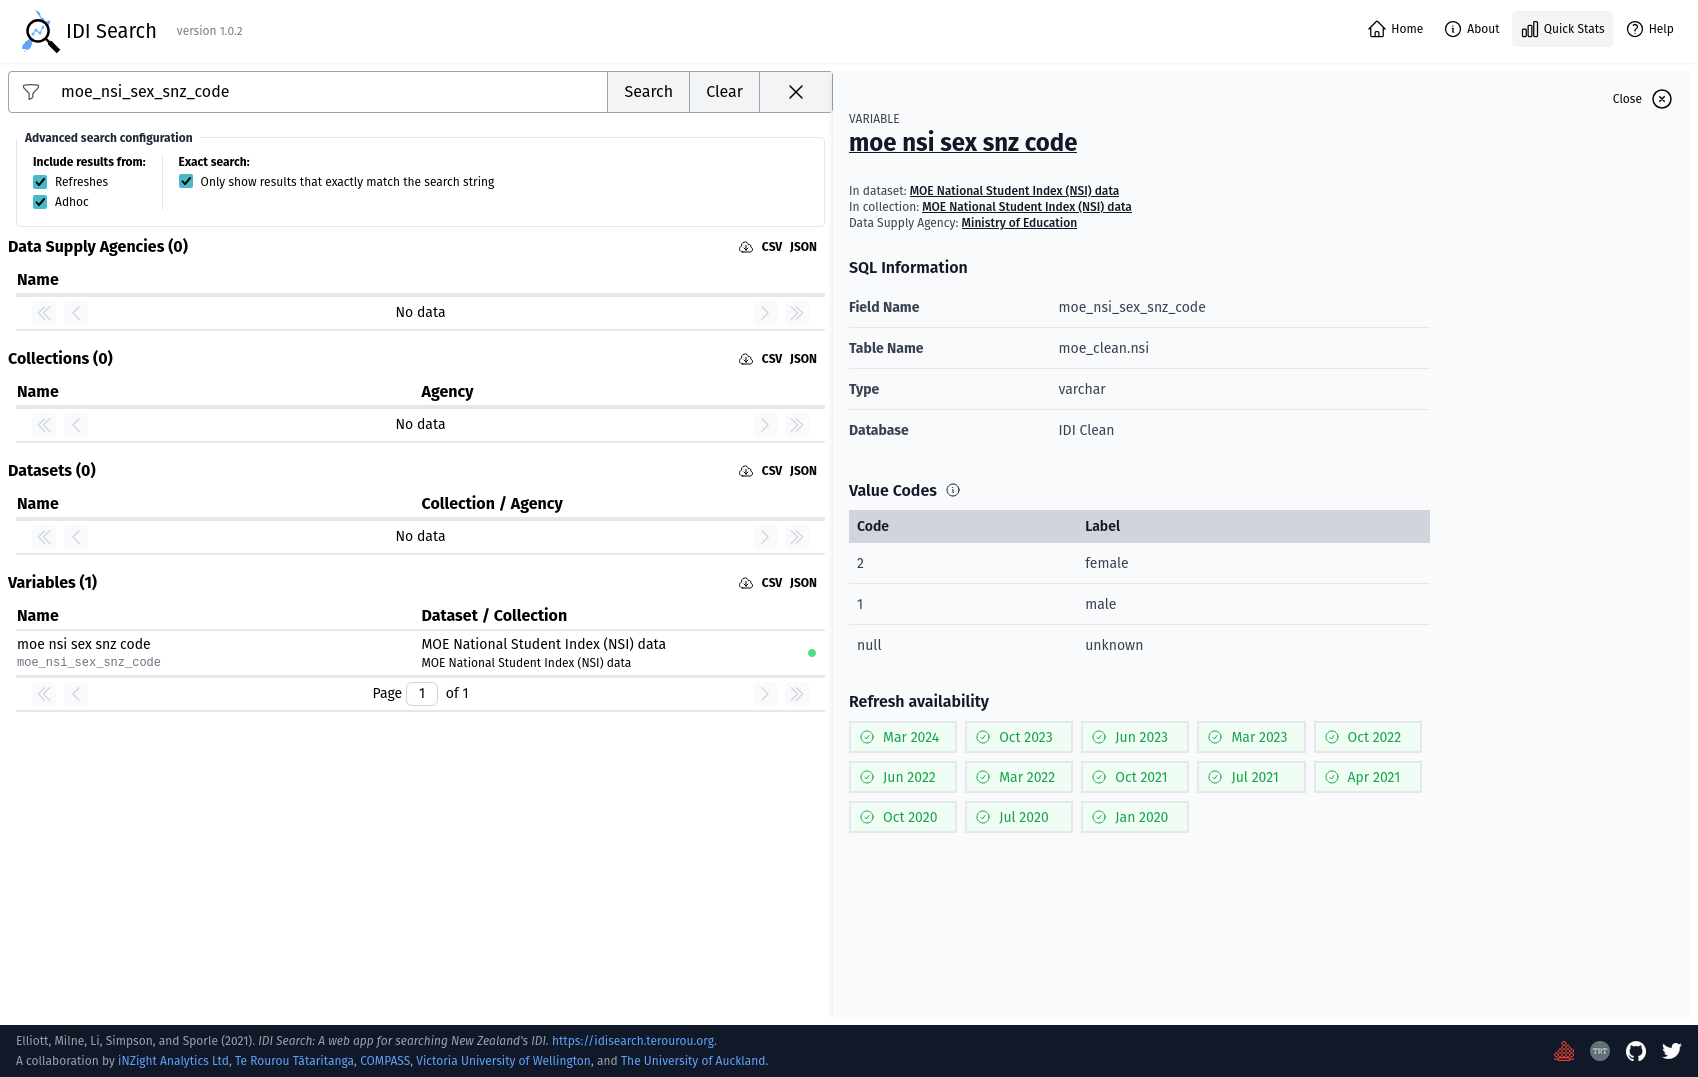
\includegraphics[keepaspectratio,
            width=\paperwidth,
            height=\paperheight]{demo4.png}
            };
    \end{tikzpicture}
\end{frame}
}

\section{Summary}

\begin{frame}
    \frametitle{Outcomes}

    \begin{itemize}
        \item 10-30 users per day (~200 users per month)
        \item Listed by Stats NZ as a go-to resource
    \end{itemize}

    \vspace{2em}
    
\includegraphics[width=\linewidth]{conc1.png}

\end{frame}

\begin{frame}
    \frametitle{Outcomes}

    \begin{itemize}
        \item Low-cost hosting funded by Stats NZ
        \item Easily updatable when new dictionaries, refreshes available
        \item Data dictionary coverage increased, quality improved
    \end{itemize}

    \begin{columns}
        \begin{column}{0.5\textwidth}
            \begin{center}
                Variables:\\[1em]
    
\includegraphics[width=\linewidth]{dd-cov1.png}
            \end{center}
        \end{column}
        \begin{column}{0.5\textwidth}
            \begin{center}
                Datasets:\\[1em]
                
\includegraphics[width=\linewidth]{dd-cov2.png}
            \end{center}
        \end{column}
    \end{columns}





\end{frame}

\begin{frame}
    \frametitle{Next steps}

    \begin{itemize}
        \item Automate data dictionary update/processing
        \item Secure funding for ongoing, routine updates
        \item New features
        \begin{itemize}
            \item flag new datasets/variables
            \item showing additional information e.g., application codes
            \item extract information from other sheets in dictionaries
        \end{itemize}
    \end{itemize}
\end{frame}

\setbeamertemplate{headline}{}
\setbeamertemplate{footline}{}
\begin{frame}
    \begin{center}
        \textbf{Dr.~Tom Elliott}\\
        iNZight Analytics Ltd.\\
        \url{tom@inzight.co.nz} \\[2em]
        
\includegraphics[width=3cm]{idisearch}\\
        \url{idisearch.terourou.org}\\
        \url{github.com/tmelliott/idi-search-app}
    \end{center}
\end{frame}

\end{document}
